% Template for Cogsci submission with R Markdown

% Stuff changed from original Markdown PLOS Template
\documentclass[10pt, letterpaper]{article}

\usepackage{cogsci}
\usepackage{pslatex}
\usepackage{float}
\usepackage{caption}

% amsmath package, useful for mathematical formulas
\usepackage{amsmath}

% amssymb package, useful for mathematical symbols
\usepackage{amssymb}

% hyperref package, useful for hyperlinks
\usepackage{hyperref}

% graphicx package, useful for including eps and pdf graphics
% include graphics with the command \includegraphics
\usepackage{graphicx}

% Sweave(-like)
\usepackage{fancyvrb}
\DefineVerbatimEnvironment{Sinput}{Verbatim}{fontshape=sl}
\DefineVerbatimEnvironment{Soutput}{Verbatim}{}
\DefineVerbatimEnvironment{Scode}{Verbatim}{fontshape=sl}
\newenvironment{Schunk}{}{}
\DefineVerbatimEnvironment{Code}{Verbatim}{}
\DefineVerbatimEnvironment{CodeInput}{Verbatim}{fontshape=sl}
\DefineVerbatimEnvironment{CodeOutput}{Verbatim}{}
\newenvironment{CodeChunk}{}{}

% cite package, to clean up citations in the main text. Do not remove.
\usepackage{apacite}

% KM added 1/4/18 to allow control of blind submission


\usepackage{color}

% Use doublespacing - comment out for single spacing
%\usepackage{setspace}
%\doublespacing


% % Text layout
% \topmargin 0.0cm
% \oddsidemargin 0.5cm
% \evensidemargin 0.5cm
% \textwidth 16cm
% \textheight 21cm

\title{Selection of goal-consistent acoustic environments by adults and
children}




\begin{document}

\maketitle

\begin{abstract}
From birth and beyond, children are navigating a world with massive
amounts of auditory input, sometimes relevant while other times purely
noise, and must somehow make sense of it all. The early auditory
environment is critical for building skills related to speech perception
and recognition, auditory discrimination, and word learning, all of
which support future language outcomes. What are still largely unknown
are the strategies young children use to learn in even the noisiest
environments. One such strategy is environmental selection, which allows
children to seek environments that align with changing goals. In the
current paper, we examined whether both children and adults make
decisions about their environments by integrating both the auditory
information and the current goal-state. While 3- and 4-year olds
struggle with discrmininating speech streams at varying sound levels,
5-year-old children and adults can, and they use this information for
environmental selection.

\textbf{Keywords:}
active learning; auditory discrimination; auditory noise; cognitive
development
\end{abstract}

\hypertarget{introduction}{%
\section{Introduction}\label{introduction}}

Children engage with their auditory environment from birth. These
experiences support speech perception and language development. With
relevant stimuli, however, also comes noise. Noise is both ubiquitous
and unavoidable, from sounds as low as a whisper (30dB) to as high as
crowded restaurants (90dB) (Erickson \& Newman, 2017). Children struggle
with speech perception and word recognition in noisy environments, and
often require signal-to-noise (SNR) levels of 5-7dB higher than adults
listening to the same stimulus (Bjorklund \& Harnishfeger, 1990; Klatte,
Bergström, \& Lachmann, 2013). Despite this, children manage to make
sense of such a noisy world. What strategies do they use?

More than 20 million children living in the United States are exposed to
dangerous noise levels daily, and 5 million of those children suffer
from noise-induced hearing loss as a result (Viet, Dellarco, Dearborn,
\& Neitzel, 2014). Unfortunately, children of color living in urban
regions are overrepresented in these numbers (Casey et al., 2017).
Chronic exposure to noise has been correlated with poorer reading
performance, reduced short term and episodic memory, and smaller
expressive vocabularies in elementary school children (Clark, Sörqvist,
\& others, 2012; Hygge, 2019; Riley \& McGregor, 2012).Yet despite
suboptimal conditions, language acquisition, cognitive development, and
full engagement with the environment is still possible, albeit more
difficult.

Children adjust their engagement with the environment when faced with
suboptimal auditory patterns, even if this causes deleterious long- term
outcomes. Cohen, Glass, \& Singer (1973) measured the sound pressure
levels in and around a noisy Manhattan high-rise apartment complex where
8- and 9-year-old middle class students lived. Auditory discrimination
mediated the relationship between reading comprehension/ability and
auditory noise. Children exposed to higher levels of auditory noise in
the home eventually learned to filter the irrelevant auditory stimuli,
but were doing so indiscriminately, such that they were also ignoring
some important stimuli.

Given the importance of the early auditory environment and
discrimination skills, children might also learn to optimize their
auditory environments to successfully complete certain goals. For
example, you might find that reading is best done in a library, not
because of its convention (because libraries function as places to
read/check out books), but because it is a quiet space. Such a strategy
might allow children to exploit environmental variation in noise to
maximize their ability to learn in suboptimal or variable conditions. In
the current paper, we asked whether and how preschool children engage in
active selection of the auditory environment to achieve a series of
goals.

One way that both children and adults navigate such a complex world is
through active learning: choices an agent makes to shape its own
learning. The dominant approach to studying active learning has
emphasized how learners approach individual stimuli. When faced with
uncertainty, both human and machine systems can learn actively by
choosing new stimuli to query that are informative with respect to the
learner's current knowledge state (Castro et al., 2008). Infants, too,
have been shown to use active learning strategies (Ruggeri, Swaboda,
Sim, \& Gopnik, 2019; see Xu, 2019 for review).

Although most active learning research has focused on stimulus
selection, perhaps children and adults are engaging in active learning
by also making decisions about the environments in which they learn. In
practice, this behavior may present itself as moving to a different room
to study for an upcoming exam or playing in a room with other children
who seem to be having the kind of fun you desire. We might expect humans
to seek out environments that best support their goals, and observe this
strategy even in young children.

In the current paper, we asked whether children and adults actively
select their auditory environment to achieve a series of goals. We
conducted two experiments with both children and adults. Although our
primary interest is whether and how children engage in environmental
selection, we also collected adult samples to offer comparisons of how
cognitively mature individuals might respond to these tasks. To ensure
that the stimuli we use can be discriminated by children in our target
ages, Experiments 1a and 1b investigate children and adults' auditory
discrimination of noise in long speech streams. Experiments 2a and 2b
then examine whether children and adults select auditory environments
that match their goals.

\hypertarget{experiment-1a}{%
\section{Experiment 1a}\label{experiment-1a}}

Previous research has consistently shown that adults can discriminate
when two different sounds are at or below 5db apart, and children as
young as four perform similarly to adults as low as 5db (Jensen \& Neff,
1993). However, the stimuli commonly used to measure auditory (or
intensity) discrimination tend to be short tonal bursts. This might
differ considerably from children's real-world auditory experiences,
which are not always transient and which may reflect more chronic noise
exposure. Additionally, noise exposure is not limited to nonspeech
signals, so the stimuli we present in experimental sessions ought to
reflect children's true encounters in their typical environments. As
such, we played participants longer speech streams of up to 25s to
determine whether their auditory discrimination skills hold under more
complex constraints. We then asked participants to select the louder
stimuli in a binary forced-choice paradigm.

\hypertarget{methods}{%
\subsection{Methods}\label{methods}}

\hypertarget{participants}{%
\subsubsection{Participants}\label{participants}}

Experiment 1a measured adults' sensitivity to 5 SNR auditory signals of
long speech streams. A total of 40 adults (mean age = 27.68 years;
52.5\% Caucasian/White) living in the United States at the time of test
were recruited to participate via the online platform, Prolific. Testing
was restricted to a laptop, desktop, or tablet. All participants were
fluent in English and had no severe visual or cognitive impairments.
Informed consent was collected from each participant before the
experiment began.

\hypertarget{materials-and-procedure}{%
\subsubsection{Materials and Procedure}\label{materials-and-procedure}}

\begin{CodeChunk}
\begin{figure}[ht]

{\centering 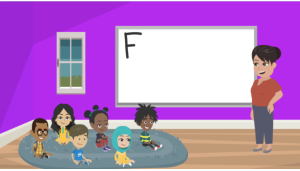
\includegraphics{figs/e1-stimuli-1} 

}

\caption[One of 10 animated classrooms participants viewed during the session]{One of 10 animated classrooms participants viewed during the session.}\label{fig:e1-stimuli}
\end{figure}
\end{CodeChunk}

Participants were told that they would watch 25-second animated videos
from each of the ten classrooms in The Alphabet School, a fictional
preschool program in which each class learns one letter of the alphabet
from A-J. Each classroom consisted of 5-6 preschool children and one
adult teacher with stereotypical male or female presentations. The wall
colors of each classroom identified which classroom participants were
viewing. In each video, the teacher would tell the students which letter
of the alphabet they would be learning, followed by three images on a
whiteboard of animals or objects that begin with that letter. Figure
@ref(fig:e1-stimuli) illustrates one of the ten classrooms shown during
the session.

Participants viewed two videos per trial, for a total of five trials.
Importantly, the classrooms differed in their signal-to-noise ratios
(SNR), which ranged from 5-25dB. Each teacher's speech was registered at
65dB, and the background noise, a recording of live preschool classrooms
collected by the first author, were equalized on speech subtracting any
silence in the clips, and ranged from 35-60dB. As such, the two videos
for each trial differed from 5-25dB from each other. The SNR levels of
each classroom were counterbalanced across conditions. At the end of
each trial, participants indicated which classroom was the louder of the
two. To ensure that participants understood the referent of the
question, we also asked at the end of the experiment whether the term
``louder'' referred to the loudness of the speaker or the loudness of
the background noise. Additionally, to reduce participant inattention in
the data, we included two attention check questions and excluded
participants who answered at least one question incorrectly.

\hypertarget{results-and-discussion}{%
\subsection{Results and Discussion}\label{results-and-discussion}}

\begin{CodeChunk}
\begin{figure}[t]
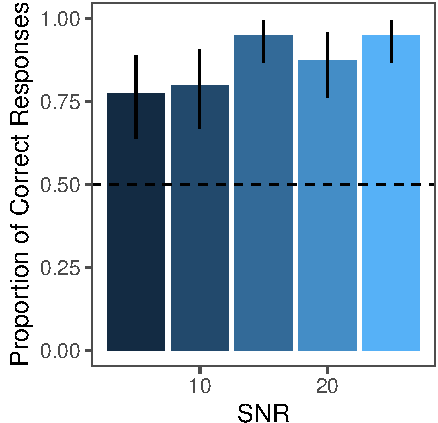
\includegraphics{figs/e1a-bar-1} \caption[Results from Experiment 1a]{Results from Experiment 1a. Proportion of correct responses across SNR levels from 5--25dB. Error bars show 95\% confidence intervals.}\label{fig:e1a-bar}
\end{figure}
\end{CodeChunk}

Given prior data, we expected that across SNR levels, adults would
correctly identify relative differences in the auditory environments
presented in this experiment. We preregistered a Bayesian mixed-effects
logistic regression predicting correct responding as a function of SNR,
with a maximal random effect structure (random slopes by SNR and a
random intercept by participant). SNR level was centered at 15 dB. On
average, adults were above chance across all five SNR levels (intercept:
\(\beta\) = 2.15, 95\% Crl = {[}1.64 - 2.9{]}), and there was a modest
effect of SNR on performance (intercept: \(\beta\) = 0.08, 95\% Crl =
{[}0.02 - 0.16{]}). Data are shown in Figure @ref(fig:e1a-bar).

This finding is both a replication of previous studies which have found
similar performance levels in adults, as well as an extension that
revealed these findings hold even with more complex stimuli. These
results affirm adults' auditory discrimination skills are fully mature,
and that they possess the cognitive resources necessary to successfully
complete this task. This study also offers a set of comparison data for
Experiment 1b, which will test the same phenomenon in young children.

\hypertarget{experiment-1b}{%
\section{Experiment 1b}\label{experiment-1b}}

\hypertarget{methods-1}{%
\subsection{Methods}\label{methods-1}}

\hypertarget{participants-1}{%
\subsubsection{Participants}\label{participants-1}}

Experiment 1b measured children's sensitivity to 5 SNR auditory signals
of long speech streams. 36 children (mean age = 4 years, 41.7\%
Caucasian/White) completed the same task as adults in Experiment 1a with
a few notable differences. Those whose caregivers indicated they heard
English at home less than 75\% of the time were excluded from analysis.

\hypertarget{materials-and-procedure-1}{%
\subsubsection{Materials and
Procedure}\label{materials-and-procedure-1}}

Children were tested synchronously over the Zoom platform by an
undergraduate research assistant. The researcher first collected
informed consent from the caregiver, who was often present but
instructed not to engage during the session, followed by assent from the
child. Children whose caregivers pointed to the computer screen or
provided answers during the session were excluded from analysis. Due to
the age range of interest, the experiment was presented strictly though
images and videos, and the research assistant verbally explained each
slide to the children. Between trials, children were rewarded with
virtual gold stars, which also served to pace the experiment and to
maintain engagement. Finally, children were not asked to identify the
referent of the question.

\hypertarget{results-and-discussion-1}{%
\subsection{Results and Discussion}\label{results-and-discussion-1}}

\begin{CodeChunk}
\begin{figure*}[H]

{\centering 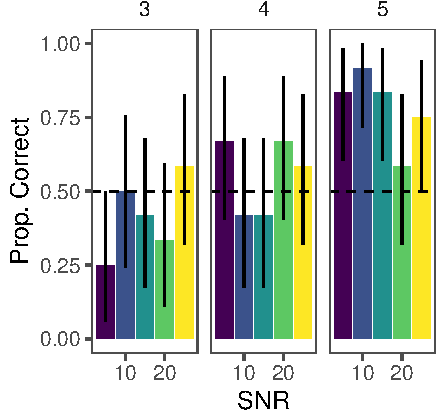
\includegraphics{figs/e1b-bar-1} 

}

\caption[Experiment 1b]{Experiment 1b. Proportion of correct responses across SNR levels from 5--25dB. Error bars show 95\% confidence intervals.}\label{fig:e1b-bar}
\end{figure*}
\end{CodeChunk}

We anticipated that, while the strength of the effect would increase
with age, all children would correctly identify relative differences in
SNRs from 10-25dB, and that only three-year-old children would be unable
to correctly identify this difference at 5dB. We ran the same Bayesian
logistic regression presented in Experiment 1a, but entered in age
(centered at the mean) as a main effect. Figure @ref(fig:e1b-bar)
demonstrates a similar, though much weaker, pattern of auditory
discrimination skills in preschool children. In the aggregate,
3-5-year-old children showed some discrimination ability on the current
paradigm (intercept : \(\beta\) = -4.51, Crl = {[}-6.76 - -2.41{]}), but
independent of SNR (intercept : \(\beta\) = 0.15, Crl = {[}-0.11 -
0.43{]}).

As expected, age plays a much larger role in these results than it does
for adults. As such, we binned the data by age {[}3;0-3;11, 4;0-4;11,
and 5;0-5;11 years{]} and ran the same analysis. Figure 4 illustrates an
age effect, such that older children were more likely to correctly
discriminate auditory signals than younger children (intercept :
\(\beta\) = -3.14, Crl = {[}-4.9 - -1.52{]}).

While these findings diverge from previous work, there is no cause for
concern. As described earlier, this task is much more challenging, and
likely requires pooling more cognitive resources, which very young
children don't yet possess. Additionally, the type of stimuli presented
here differs from the tonal bursts or other brief nonspeech sounds used
in earlier work. Taken together, our findings may expose some of the
limits of auditory discrimination abilities in preschool children.

\hypertarget{experiment-2a}{%
\section{Experiment 2a}\label{experiment-2a}}

If participants can successfully discriminate between sound pressure
levels, do they then use this information to inform which goals are most
appropriate in these environments? Participants watched a video of a
third-person character with several goals and were asked to select the
environment that he should complete these goals. We hypothesized that
adults would both consistently discriminate even the most challenging
auditory signals given their mature cognitive system, and that children
would show a developmental trajectory in both auditory discrimination
and environmental selection. In other words, older children would
perform similarly to adults on the auditory discrimination task and
would show weaker, though similar performance on the environmental
selection task.

\hypertarget{methods-2}{%
\subsection{Methods}\label{methods-2}}

\hypertarget{participants-2}{%
\subsubsection{Participants}\label{participants-2}}

1024 adults (mean age = 27.82 years; 69.5\% Caucasian/White) living in
the United States at the time of test were recruited to participate via
the online platform, Prolific. Testing was restricted to a laptop,
desktop, or tablet. All participants were fluent in English and had no
severe visual or cognitive impairments. Informed consent was collected
from each participant before the experiment began.

\hypertarget{materials-and-procedure-2}{%
\subsubsection{Materials and
Procedure}\label{materials-and-procedure-2}}

Participants were introduced to a preschool-aged character named Ryan
with eight goals to complete throughout the experiment- (1) to read a
book, (2) to build a tower out of blocks, (3) to learn the letters of
the alphabet, (4) to paint a picture, (5) to dance to his favorite
music, (6) to learn a new language called Zerpie, (7) to talk to a
friend, and (8) to eat lunch. All activities had relatively simple
explanations with the exception of (6). For this trial, participants
were told that Ryan's new neighbor, Logan, speaks a rare language called
Zerpie, a language he doesn't speak. Ryan wants to learn Zerpie so he
can communicate with Logan. For all activities, Ryan must complete each
task in a closed room. Each goal was presented individually as a single
trial for a total of eight trials. In each trial, participants watched a
video in which Ryan stood in between two closed doors labeled ``A'' and
``B'', respectively. Before the video began, participants were told to
watch and listen carefully to decide in which of the two rooms Ryan
should complete his goal. As in Experiment 1, we manipulated the sound
level of each room, but removed any classroom stimuli, including the
teacher, and only allowed one child to open and stand in front of each
door. As such, participants did not have access to any visual
information of the room, and could only rely on auditory information, as
well as any information provided by the character who opened the door.
Each character's voice was equalized to 65dB and, unlike in Experiment
1, all characters shared the same voice. All characters except Ryan were
preschool girls but differed in appearance. The same background noise in
Experiment 1 was used for the current experiment, and the difference in
SNR between the two rooms was 5-25dB. During the video, each character
would open their respective door beginning with Room A. The character in
Room A always said, ``You can {[}goal{]} in this room'', while the
character in Room B always said, ``Or you can {[}goal{]} in this room.''
While the room on the left was always labeled ``A'' and the room on the
right was always labeled ``B'', the characters from and sound levels of
each room, as well as goal order were counterbalanced across conditions.
For each trial, participants were told which goal Ryan wanted to
complete and were asked to select the room that he should complete his
goal. After making a selection, they were then asked to briefly explain
their choice. Responses for the quieter room (relative to the other and
based on the actual sound pressure level) were given a 1, while
responses for the louder room were given a 0.

\hypertarget{results-and-discussion-2}{%
\subsection{Results and Discussion}\label{results-and-discussion-2}}

We expected that adults would overwhelming select the quieter room when
the goal was (1) to read a book, (2) to learn the new language called
Zerpie, and (3) to learn the letters of the alphabet, but would be more
likely to select the louder room when the goal was (1) to dance to his
favorite music, (2) to talk to a friend, and (3) to build a tower out of
blocks. Additionally, we expected participants to have no sound level
preference for (1) eating lunch and (2) painting a picture. This is
because the latter two activities might be more ambiguous in the degree
to which a relatively quieter or louder environment supports or hinders
the goal. We preregistered the following Bayesian mixed-effects logistic
regression:\\
quiet \textasciitilde{} activity + (activity \textbar{} subject\_id),
where quiet refers to the number of times the quiet room was selected as
the response, and both the activity in which participants were exposed
and participants' individual responses were entered as random effects in
the model. Figure 5 depicts adult participants' preferences for quieter
environments based on the chosen activity. Activities had a marginal
effect on room selection (intercept: \(\beta\) = 0.07, Crl = {[}-0.3 -
0.45{]}) We found that all but two activities were either preferred in
the quiet or loud room- eating (intercept : \(\beta\) = 0.1, Crl =
{[}-0.5-0.8{]}) and talking (intercept : \(\beta\) = 0.5, Crl =
{[}-0.06-1.2{]}), which were almost equally preferred in both rooms.
Reading was most preferred in the quiet room while dancing was most
preferred in the loud room.

\begin{CodeChunk}
\begin{figure}[H]

{\centering 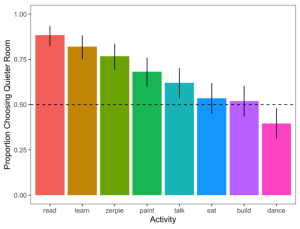
\includegraphics{figs/image 5-1} 

}

\caption[Experiment 2a]{Experiment 2a. Proportion of participants selecting the quieter room by activity. Values closer to 1 on the y-axis indicate a preference for the quiet room.}\label{fig:image 5}
\end{figure}
\end{CodeChunk}

These findings suggests adults are not only sensitive to differences in
the auditory environment, but they also use these cues to reach certain
goals. Moreover, adults are not indiscriminately selecting the quieter
environment, but are instead taking into account the intention and
explicitly weighing the auditory environment to do so.

\hypertarget{experiment-2b}{%
\section{Experiment 2b}\label{experiment-2b}}

In the next next study, we asked the extent to which 5-year-old children
also weigh auditory information and goal-seeking to make decisions about
optimal environments.

\hypertarget{methods-3}{%
\subsection{Methods}\label{methods-3}}

\hypertarget{participants-3}{%
\subsubsection{Participants}\label{participants-3}}

{[}final number{]} 5-year-old children (mean age = 63.95 months, \%\%
Caucasian/White) completed a truncated version of Experiment 2a to both
prevent testing fatigue and to maximize any response differences based
on the presented goals. In addition to testing children on the Zoom
platform, we also recruited a small group of children at a Bay Area
nursery school, which serves children 2-5 years old. This in-person
testing was conducted with both caregiver consent and participant
assent. As with the online testing, participants must have heard English
at home at least 75\% of the time and must have no cognitive, visual, or
neurological concerns. Given the finding from Experiment 1b that 3- and
4-year-old children performed near chance in the auditory discrimination
task with long speech streams, we chose to only test 5-year-old children
for this portion of the study.

\hypertarget{materials-and-procedure-3}{%
\subsubsection{Materials and
Procedure}\label{materials-and-procedure-3}}

We tested children on the four activities with the widest differences
observed in Experiment 2a- (1) to read a book, (2) to learn the letters
of the alphabet, (3) to build a tower out of blocks, and (4) to dance to
the music, a total of four trials. Additionally, participants in this
experiment were only shown videos in which the two rooms had SNR
differences of 25dB. This is because 5-year-old performance in
Experiment 1b did not differ by SNR. The rooms and characters remained
consistent with Experiment 2a, with one exception: the room labels,
``A'' and ``B'', were replaced with one black circle for Room 1 and two
black circles for Room 2.. This change was implemented after finding
that several participants in the pilot study seemed to favor the letter
A over B, and because these letter labels may interfere with responses
when the goal is to learn the letters of the alphabet. Black circle
labels, on the other hand, are more abstract and may reduce this bias.
As done previously, the characters, sound pressure levels, and goal
order were counterbalanced across conditions. Whether testing online or
in-person, participants were shown the same set of videos and a research
assistant (for online testing) or the first author (for in-person
testing) verbally explained each slide and video to participants. After
watching each video, participants were asked to select the room Ryan
should complete his goal and to briefly explain their response. As in
Experiment 2a, responses for the quieter room (relative to the other and
based on the actual sound pressure level) were given a 1, while
responses for the louder room were given a 0.

\hypertarget{results-and-discussion-3}{%
\subsection{\texorpdfstring{\textbf{Results and
Discussion}}{Results and Discussion}}\label{results-and-discussion-3}}

\begin{CodeChunk}
\begin{figure}[H]

{\centering 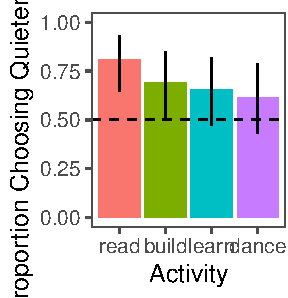
\includegraphics{figs/unnamed-chunk-3-1} 

}

\caption[Experiment 2b]{Experiment 2b. Proportion of participants selecting the quieter room by activity.}\label{fig:unnamed-chunk-3}
\end{figure}
\end{CodeChunk}

We expected to see a similar, though weaker, response pattern as adult
participants in Experiment 2a. Figure 6 depicts childrens' preferences
for quieter environments based on the chosen activity. We ran the same
logistic regression as in Experiment 2a, but added age as a main effect.
As expected, children were more likely to select the quieter room for
book reading and learning the letters of the alphabet.

These findings propose that 5-year-old children are using a separate
strategy from adults by selecting the quieter room more often regardless
of the goal.

\hypertarget{general-discussion}{%
\section{General Discussion}\label{general-discussion}}

These set of experiments demonstrate both an important relationship
between auditory discrimination and a strategy children and adults use
to optimize their auditory environments and achieve goals. Experiment 1a
and 1b found that adults and older children can sufficiently
discriminate auditory stimuli in long speech streams at sound pressure
levels as low as 5dB. The challenge we observed in 3- and 4-year-old
children's performance may reveal a lack of cognitive skills necessary
to complete the task. The fact that 5-year-old children were performing
above chance, however, may indicate that these skills are rapidly
maturing by the fifth year of life. Experiment 2a displayed adult's
selectivity of auditory environments based on changing goals while
Experiment 2b demonstrated the opposite; 5-year-olds were more likely to
select the quieter room regardless of the stated goal.

The latter finding does not necessarily reveal a failure on children's
end, but rather a useful heuristic they might employ when they are still
learning about much of their world. Whereas most adults have the
flexibility of basic linguistic and cognitive mastery to seek louder
environments for certain tasks, children can reduce uncertainty by
selecting quieter auditory environments and then focus their attention
and cognitive energy on achieving them. Previous work has shown that
humans (including children) have an intrinsic desire to reduce
uncertainty (Gottlieb, Oudeyer, Lopes, \& Baranes, 2013). In the wild,
children pursue ways to reduce uncertainty when faced with a possible
reward (Feldstein \& Witryol, 1971) and search for additional
information on a particular topic when their intuitive theories are less
informative (Wang, Yang, Macias, \& Bonawitz, 2021). Thus, this
experiment may offer another example of uncertainty reduction in
children.

By understanding the strategies children use to learn in noisy auditory
environments, we might offer better solutions for those exposed to
chronic noise, thereby mitigating some of its negative effects. This is
becoming more and more critical as cities become more populated
(bringing construction with it) and auditory noise becomes even more
unavoidable. Future studies will need to (1) explore the developmental
trajectory of environmental selection such that we can identify when
indiscriminately selecting the quieter environment is no longer
beneficial, and (2) examine the boundaries of environmental selection by
probing these questions with other goals and in other contexts
(e.g.~first-person goal-setting). Investigating how children learn in
noise will ultimately bring us closer to understanding the complex
wonders of childhood.

\hypertarget{acknowledgements}{%
\section{Acknowledgements}\label{acknowledgements}}

Retracted for anonymous submission

\hypertarget{references}{%
\section{References}\label{references}}

\setlength{\parindent}{-0.1in} 
\setlength{\leftskip}{0.125in}

\noindent

\hypertarget{refs}{}
\leavevmode\hypertarget{ref-bjorklund1990}{}%
Bjorklund, D. F., \& Harnishfeger, K. K. (1990). The resources construct
in cognitive development: Diverse sources of evidence and a theory of
inefficient inhibition. \emph{Developmental Review}, \emph{10}(1),
48--71.

\leavevmode\hypertarget{ref-casey2017}{}%
Casey, J. A., Morello-Frosch, R., Mennitt, D. J., Fristrup, K., Ogburn,
E. L., \& James, P. (2017). Race/ethnicity, socioeconomic status,
residential segregation, and spatial variation in noise exposure in the
contiguous united states. \emph{Environmental Health Perspectives},
\emph{125}(7), 077017.

\leavevmode\hypertarget{ref-castro2008}{}%
Castro, R. M., Kalish, C., Nowak, R., Qian, R., Rogers, T., \& Zhu, X.
(2008). Human active learning. In \emph{Advances in neural information
processing systems} (pp. 241--248). Citeseer.

\leavevmode\hypertarget{ref-clark20123}{}%
Clark, C., Sörqvist, P., \& others. (2012). A 3 year update on the
influence of noise on performance and behavior. \emph{Noise and Health},
\emph{14}(61), 292.

\leavevmode\hypertarget{ref-cohen1973}{}%
Cohen, S., Glass, D. C., \& Singer, J. E. (1973). Apartment noise,
auditory discrimination, and reading ability in children. \emph{Journal
of Experimental Social Psychology}, \emph{9}(5), 407--422.

\leavevmode\hypertarget{ref-erickson2017}{}%
Erickson, L. C., \& Newman, R. S. (2017). Influences of background noise
on infants and children. \emph{Current Directions in Psychological
Science}, \emph{26}(5), 451--457.

\leavevmode\hypertarget{ref-feldstein1971}{}%
Feldstein, J. H., \& Witryol, S. L. (1971). The incentive value of
uncertainty reduction for children. \emph{Child Development}, 793--804.

\leavevmode\hypertarget{ref-gottlieb2013}{}%
Gottlieb, J., Oudeyer, P.-Y., Lopes, M., \& Baranes, A. (2013).
Information-seeking, curiosity, and attention: Computational and neural
mechanisms. \emph{Trends in Cognitive Sciences}, \emph{17}(11),
585--593.

\leavevmode\hypertarget{ref-hygge2019}{}%
Hygge, S. (2019). Noise and cognition in children.

\leavevmode\hypertarget{ref-jensen1993}{}%
Jensen, J. K., \& Neff, D. L. (1993). Development of basic auditory
discrimination in preschool children. \emph{Psychological Science},
\emph{4}(2), 104--107.

\leavevmode\hypertarget{ref-klatte2013}{}%
Klatte, M., Bergström, K., \& Lachmann, T. (2013). Does noise affect
learning? A short review on noise effects on cognitive performance in
children. \emph{Frontiers in Psychology}, \emph{4}, 578.

\leavevmode\hypertarget{ref-riley2012}{}%
Riley, K. G., \& McGregor, K. K. (2012). Noise hampers children's
expressive word learning.

\leavevmode\hypertarget{ref-ruggeri2019}{}%
Ruggeri, A., Swaboda, N., Sim, Z. L., \& Gopnik, A. (2019). Shake it
baby, but only when needed: Preschoolers adapt their exploratory
strategies to the information structure of the task. \emph{Cognition},
\emph{193}, 104013.

\leavevmode\hypertarget{ref-viet2014}{}%
Viet, S. M., Dellarco, M., Dearborn, D. G., \& Neitzel, R. (2014).
Assessment of noise exposure to children: Considerations for the
national children's study. \emph{Journal of Pregnancy and Child Health},
\emph{1}(1).

\leavevmode\hypertarget{ref-wang2021}{}%
Wang, J., Yang, Y., Macias, C., \& Bonawitz, E. (2021). Children with
more uncertainty in their intuitive theories seek domain-relevant
information. \emph{Psychological Science}, \emph{32}(7), 1147--1156.

\leavevmode\hypertarget{ref-xu2019}{}%
Xu, F. (2019). Towards a rational constructivist theory of cognitive
development. \emph{Psychological Review}, \emph{126}(6), 841.

\bibliographystyle{apacite}


\end{document}
